\chapter{Database \& Data Center Security}
%% è a pagina 128
%% TODO: ricontrollare TUTTO è pieno di ripetizioni !!
\section{Introduzione} %% TODO: vedere se mantenere la section o toglierla

Negli ultimi anni il modello di Database Relazionale è diventato molto popolare ed ampiamente utilizzato da
privati e aziende.
Per molte organizzazioni, è importante essere in grado di
fornire a clienti, partner e dipendenti l'accesso alle informazioni da loro memorizzate. Ma tali
informazioni possono essere prese di mira da minacce interne ed esterne, possono essere utilizzate
impropriamente o modifiche da entità non autorizzate. Di conseguenza, la sicurezza
specificamente adattata ai database è una componente sempre più importante di una strategia generale per la protezione dei dati.

Di seguito andremo ad elencare le principali ragioni per cui la sicurezza dei database non ha tenuto il passo con
l'aumento della dipendenza dai database:

\begin{enumerate}
    \item C'è un drammatico squilibrio tra la complessità dei moderni
          database (DBMS) e le tecniche di sicurezza usate per proteggere questi
          sistemi critici. Un DBMS è un software molto complesso e di grandi
          dimensioni, che fornisce molte opzioni, che devono essere tutte ben
          comprese e poi protette per evitare violazioni dei dati.
    \item I database hanno un sofisticato protocollo di interazione chiamato
          \textit{Structured Query Structured Query Language} (\textbf{SQL}),
          che è molto complesso e potente, quindi deve essere appreso pienamente
          prima di poter essere utilizzato.
    \item La mancanza di personale specializzato. L'azienda media non ha
          personale addetto alla gestione della sicurezza di database.
          Generalmente hanno uno staff per la sola amministrazione del DB che
          non è sufficientemente formato per gestirne anche la sicurezza.
    \item La maggior parte degli ambienti aziendali consiste in una miscela
          eterogenea di piattaforme di database, piattaforme aziendali e OS,
          quindi non avere un solo db o un solo tipo di sistema operativo
          rappresenta una problematica che crea un'ulteriore complessità per il
          personale.
    \item La crescente dipendenza dalla tecnologia cloud per ospitare parte o
          tutto il database aziendale risulta essere un'ulteriore sfida in quanto
          aggiunge ulteriori oneri per il
          personale di sicurezza.
\end{enumerate}

Possiamo definire quindi un \textbf{Database} come una raccolta strutturata di
dati immagazzinati e messi in relazione tra di loro per essere utilizzati da una
o più applicazioni; organizzati in tabelle che possono essere manipolate tramite
un apposito linguaggio chiamato Data Definition Language (\textbf{DDL}); recuperati
tramite un apposito linguaggio di query standardizzato (\textbf{SQL}) e gestiti
da un apposito software chiamato \textbf{Database Management System}.\\

Il principale vantaggio dei Database, oltre alla possibilità di organizzare e
recuperare informazioni in pochissimo tempo, è quella di poter limitare l'accesso
e la visibilità solo a singole parti di un determinato file. Nei classici sistemi
operativi questo non risulta possibile dato che si può solo specificare se un
utente può o no accedere ad un file ma non limitarne la visibilità solo ad una
sua parte.

\section{SQL Injection Attack}

Gli attacchi di tipo SQL Injection sono una delle minacce alla sicurezza diffuse
e pericolose. Questo attacco si basa sull'invio di dati contenenti una
parte di query malevola per l'estrazione, modifica o cancellazione di tutti i
dati presenti all'interno di un database fruibile tramite un'applicazione web.

\begin{figure}[H]
    \centering
    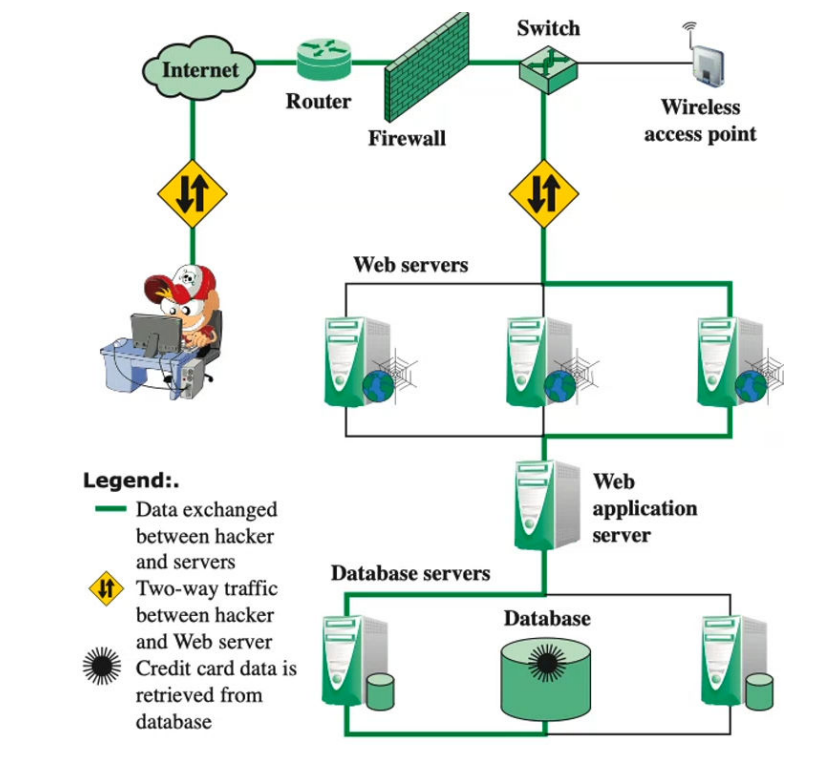
\includegraphics[width=10cm, keepaspectratio]{capitoli/sql_security/imgs/sql1.png}
    \caption{Esempio di un tipico attacco SQL Injection.}
\end{figure}

Questo attacco funziona tipicamente terminando prematuramente una stringa di
testo, generalmente con un commento \verb|--|, e aggiungendo un nuovo comando
che verrà eseguito dal database ed impedirà l'esecuzione del resto della query.\\

Possiamo caratterizzare gli attacchi SQL Injection in termini di via d'attacco e
tipo di attacco.

\subsection{Attack Avenues}

Le principali vie d'attacco sono le seguenti:

\paragraph{Input dell'utente:}
l'aggressore fornisce al database un input opportunamente modificato per
forzare l'esecuzione di una query malevola.

\paragraph{Variabili server:}
Le variabili del server sono un insieme di variabili che contengono intestazioni
HTTP, intestazioni del protocollo di rete e variabili ambientali. Le
applicazioni web usano queste variabili del server in una varietà di modi, come
la registrazione di statistiche e informazioni di utilizzo per identificare le
tendenze di un utente. Se queste variabili sono registrate in un database senza
sanificazione, questo potrebbe creare una vulnerabilità di SQL injection in
quanto è possibile modificarle ed inserirci codice arbitrario.

\paragraph{Second Order Injection:}
Un attaccante può sfruttare dati già presenti nel sistema o nel database per
attivare un attacco SQL Injection cosicché quando avviene effettivamente
l'attacco la query malevola non proviene dall'utente ma direttamente dal sistema
stesso.

\paragraph{Cookie:}
Di solito vengono utilizzati anche i cookie per creare in modo automatico query
per salvare dati o manipolarli. Un attaccante può modificare il contenuto di un
cookie per andare a forzare l'esecuzione di una query maligna all'interno di un
database.

\paragraph{Input fisico dell'utente:}
Gli attacchi SQL Injection possono anche avvenire all'esterno di una richiesta
web: prendiamo in considerazione un sistema che in automatico scannerizza e
archivia documenti tramite l'ausilio di modelli di machine learning, questo può
essere attaccato scrivendo fisicamente una query malvagia all'interno del
documento da acquisire.


\subsection{Attack Types} %% a pagina 135


%% continuare fino a pagina 138